\section{Bremse 4.0}
Die Bremse 4.0 blabla 
Das Druckluftschema der \gls{Bremse 4.0} ist in Abbildung \ref{fig:GW40Schema} zu sehen.\par
\begin{figure}[hbt]
    \centering
    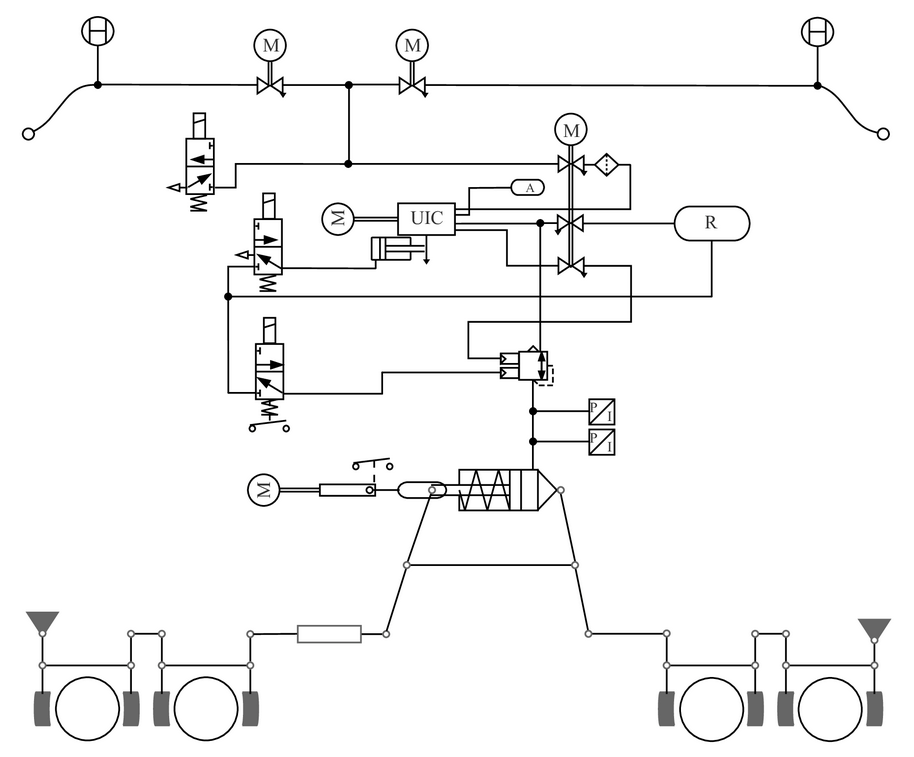
\includegraphics[width=\textwidth]{Bilder/GW40Schema.png}
    \caption{Schema der Güterwagen 4.0 Bremse - Bremse 4.0}
    \label{fig:GW40Schema}
\end{figure}
Für die FMEA-Anlyse wird eine Struktur- und Funktionsanalyse der einzelnen Bauteile benötigt. 

\subsection{Strukturanalayse}
\gls{Bremse 4.0} des Demonstrators.\par
Bauteile die Untersucht werden sollen.\par
Legende: \\
- Komponente des konventionellen \gls{Güterwagens}, die unverändert bleibt\\
+ Komponente des konventionellen \gls{Güterwagens}, die zu einer 4.0-Komponente wird\\
\** Komponente des Güterwagen 4.0, die es nicht im konventionellen Güterwagen gibt\par
\begin{itemize}
    \item[-] Hauptluftleitung
    \begin{itemize}
        \item[+] Endabsperrhahn oder Muffenkugelhahn
        \item[+] Schauzeichen (Anzeige Druck)
        \item[-] Schlauchkupplung
        \item[-] Abzweigung HL-Steuerventil
    \end{itemize}
    \item[+] Steuerventil 4.0
    \begin{itemize}
        \item[-] UIC-konformes Steuerventil
        \item[-] A-Kammer (eventuell Bestandteil des Steuerventil)
        \item[+] G/P-Umstellvorrichtung
        \begin{itemize}
            \item[+] Visuelle Zustandsanzeige mit mechanischer Umsetzung
        \end{itemize}
        \item[+] Schnelllösen
        \item[+] Bremse aus
        \begin{itemize}
            \item[+] Visuelle Zustandsanzeige mit mechanischer Umsetzung
        \end{itemize}
    \end{itemize}
    \item[-] Relaisventil\footnote{Druckübersetzung: aus $C_v$-Druck wird Leistungsdruck}
    \begin{itemize}
        \item[-] Stufenweise Lastwechselumstelleinrichtung
        \begin{itemize}
            \item[+] Visuelle Zustandsanzeige
        \end{itemize}
        \item[+] Vorsteuerventil mit Rückmeldeschalter zur Lasteinstellung\footnote{bestromt=beladen; unbestromt=unbeladen}
    \end{itemize}
    \item[\textasteriskcentered] C-Druck-Sensor\footnote{Für Bremsprobe (siehe Triebzug); Zwischen Relaisventil und Zylinder}
    \item[-] Bremsgestänge\footnote{Lastwechsel wird ausgebaut}
    \item[-] Verschleisnachsteller
    \item[+] Feststellbremse\footnote{Automatische Ablaufbremse ,öglich, Motor mit Kurbel, stetig gebremst, Anlegezeit erstmal zweitrangig}
    \begin{itemize}
        \item[+] Stellantrieb
        \item[-] mechanische Übersetzung
        \item[\textasteriskcentered] Rückmeldeschalter\footnote{für sichere Fahrt: vollständig gelöst, für sicher gebremst: angeschriebenes Handbremsgewicht wird erreicht: 10 Umdrehungen vom gelösten Zustand; dazwischen undefiniert}
        \begin{itemize}
            \item[\textasteriskcentered] Visuelle Anzeige\footnote{Weg der Spindel; Rot, undefiniert, grün}
        \end{itemize}
    \end{itemize}
    \item[\textasteriskcentered] ep-Bremsen\footnote{Entlüftet die HL lokael; elektrische Ansteuerung, indirekte ep-Bremsenfunktion - Vordermann bremst, bremse ich auch, kein ep-lösen, pneumatisches 2-Wege-Ventil}
\end{itemize}

\subsection{Funktionsanalyse}
Funktionen für Zustandsänderugnen an der \gls{Bremse 4.0}
\begin{fkt} \textbf{Feststellbremse}:
\begin{itemize}
    \item gewünschte Bremskraft herstellen / Fahrzeug an einem gewählten Ort auf eine gewünschte Geschwindigkeit verzögern
    \item Fahrzeug dauerhaft gegen wegrollen sichern
    \item lösen
\end{itemize}
\end{fkt}

\begin{fkt} \textbf{Hauptluftleitung}:
\begin{itemize}
    \item Durchleiten der Brems- und Löseanforderung
    \item Einhalten der definierten Leckrate
    \item Energieversorgung der pneumatischen Bremse
    \item Druckfreiheit der Schlauchkupplungen gewährleisten
    \item HL verbinden und absperren
\end{itemize}
\end{fkt}

\begin{fkt} \textbf{Relaisventil}:
\begin{itemize}
    \item Anpassung des Drucks an das Wagengewicht
    \item Leistungsverstärkung anzeigen
    \item Lastwechseleinstellung
\end{itemize}
\end{fkt}

\begin{fkt} \textbf{C-Druck}:
\begin{itemize}
    \item Bremszylinderdruck messen
\end{itemize}
\end{fkt}

\begin{fkt} \textbf{Bremsgestänge}:
\begin{itemize}
    \item gleichmäßige Kraftübertragung auf Räder
    \item VErschleiß nachstellen
\end{itemize}
\end{fkt}

\begin{fkt} \textbf{ep-Bremsen}:
\begin{itemize}
    \item HL lokal entlüften
    \item HL lokal absenken
\end{itemize}
\end{fkt}

\begin{fkt} \textbf{Steuerventil 4.0}
\begin{itemize}
    \item Referenzdruck vorhalten
    \item A-Kammer entlüften
    \item Füll- und Lösezeiten einstellen
    \item lokalen Druckluft-Vorrat speichern
    \item $C_v$-Druck auf $f(a, HL, t, ..)$ einstellen
    \item Steuerventil von HL trennen
    \item \gls{Bremsart} anzeigen
\end{itemize}
\end{fkt}